\documentclass[a4paper,10pt]{article}
\usepackage[left=3cm,top=3cm,right=3cm,bottom=3cm,head=4cm,includefoot]{geometry}

%%%%%%%%%%%%%%%%%%%%%%%%%%%%%%%%%%%%%%%%%%%%%%%%%%%%%%%%%%%%%%%%%%%%%%%%
% Paquetes utilizados
%%%%%%%%%%%%%%%%%%%%%%%%%%%%%%%%%%%%%%%%%%%%%%%%%%%%%%%%%%%%%%%%%%%%%%%%

% Graficos complejos
\usepackage{graphicx}
\usepackage{rotating}
\usepackage{caption}
\usepackage{subcaption}
\usepackage{placeins}

% Soporte para el lenguaje español
\usepackage{textcomp}
\usepackage[utf8]{inputenc}
\usepackage[T1]{fontenc}
\DeclareUnicodeCharacter{B0}{\textdegree}
\usepackage[spanish]{babel}

% Codigo fuente embebido
\usepackage{listings}

% PDFs embebidos para el apendice
\usepackage{pdfpages}

% Matematicos
\usepackage{amssymb,amsmath}

% Tablas complejas
\usepackage{multirow}

% Formato de parrafo
\setlength{\parskip}{1ex plus 0.5ex minus 0.2ex}

%%%%%%%%%%%%%%%%%%%%%%%%%%%%%%%%%%%%%%%%%%%%%%%%%%%%%%%%%%%%%%%%%%%%%%%%
% Titulo
%%%%%%%%%%%%%%%%%%%%%%%%%%%%%%%%%%%%%%%%%%%%%%%%%%%%%%%%%%%%%%%%%%%%%%%%

% Titulo principal del documento.
\title{\textbf{Trabajo Práctico 2: Base de datos de personas}}

% Informacion sobre los autores.
\author{\\
  Arana Andrés, \textit{P. 86.203}                                 \\
  \texttt{and2arana@gmail.com}                                     \\ [2.5ex]
  Arias Damián, \textit{P. 89.952}                                 \\
  \texttt{arias.damian@gmail.com}                                  \\ [2.5ex]
  Sergio Matias Piano, \textit{P. 85.191}                          \\
  \texttt{smpiano@gmail.com}                                       \\ [2.5ex]
                                                                   \\
  \normalsize{2do. Cuatrimestre de 2014}                           \\
  \normalsize{75.59 Técnicas de Programación Concurrente 1}        \\
  \normalsize{Facultad de Ingenieria, Universidad de Buenos Aires} \\
}
\date{}

%%%%%%%%%%%%%%%%%%%%%%%%%%%%%%%%%%%%%%%%%%%%%%%%%%%%%%%%%%%%%%%%%%%%%%%%
% Documento
%%%%%%%%%%%%%%%%%%%%%%%%%%%%%%%%%%%%%%%%%%%%%%%%%%%%%%%%%%%%%%%%%%%%%%%%

\begin{document}

% ----------------------------------------------------------------------
% Top matter
% ----------------------------------------------------------------------
\thispagestyle{empty}
\maketitle

\begin{abstract}

  Este informe sumariza el desarrollo del trabajo practico 2 de la materia
  Técnicas de Programación Concurrente I (75.59) dictada en el segundo
  cuatrimestre de 2014 en la Facultad de Ingenieria de la Universidad de Buenos
  Aires. El mismo consiste en la construcción de una aplicación de gestión de
  información de contacto de personas compuesta por un servidor de datos y
  varios clientes conectados a través de una cola de mensajes.

\end{abstract}

\clearpage

% ----------------------------------------------------------------------
% Indice
% ----------------------------------------------------------------------
\tableofcontents
\clearpage


% ----------------------------------------------------------------------
% Desarrollo
% ----------------------------------------------------------------------
%\part{parte}


\section{Análisis del problema}

\subsection{Descripción}

El sistema a desarrollar se dividirá en dos aplicaciones, una será el gestor de base de datos que se encargará de realizar las inserciones y actualizaciones de los registros y la otra será el cliente que realizará pedidos de inserción, actualización y consulta de los registros.

Los campos de los registros tendrán que ser validados al momento de su ingreso para que su tamaño se matenga dentro de los límites impuestos.

Como requisitos adicionales la base de datos se deberá almacenar en un archivo cada vez que el gestor se cierre y, por otro lado, el gestor de la base deberá poder atender consultas de múltiples clientes al mismo tiempo.

\subsection{Casos de uso}

	\begin{center}
        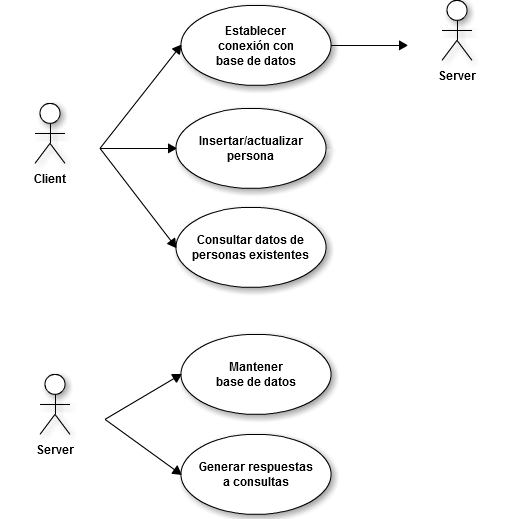
\includegraphics[scale=0.8]{casos_de_uso.png}
    \end{center}
    
\clearpage
\section{Desarrollo de la solución}

\subsection{Hipótesis y alcance}

\begin{itemize}
\item El gestor de base de datos no soporta la operación de borrado de registros.
\item No se pueden consultar personas por su dirección o su teléfono.
\item Los clientes no reciben confirmación luego de modificar o insertar un registro en la base de datos.
\end{itemize}

\subsection{Procesos}

\begin{itemize}
\item \textbf{server}: este proceso se encarga de leer el archivo completo que representa a la base de datos y mapea todos sus registros en memoria. Todas las modificaciones y lecturas a la base de datos se harán directamente en memoria y se guardará su estado en disco recién cuando se cierre el servidor.
Lo siguente que hará el servidor será crear una nueva cola de mensajes pidiendolé su identificador al kernel.
Una vez finalizada la etapa de inicialización, el servidor escucha la cola de mensajes esperando la conexión de los clientes y respondiendo consultas de los ya conectados.

\item \textbf{client}: podrá haber varias instancias de este proceso corriendo en el sistema al mismo tiempo. En el momento de su creación se le pasará por parámetro el identificador de la cola de mensajes a la que se deba subscribir (el identificador es informado por el servidor al momento de su creación).
Una vez subscripta a la cola de mensajes cada cliente otendrá un identificador único por parte del servidor con el cual podrán leer y escribir los mensajes.

\end{itemize}

\subsection{Resolución de casos de uso}

\begin{itemize}
\item \textbf{Establecer conexión con base de datos}: el establecimiento de la conexión implica que tanto el cliente como el servidor conocen el identificador de la cola de mensajes del sistema y que además los clientes tiene un id asignado por el servidor que se genera en forma incremental a medida que se van conectando clientes.

\item \textbf{Insertar/actualizar persona}: el cliente puede pedir la inserción o actualización de un registro particular especificando en id que éste tiene en la base de datos, para esto el usuario deberá ingresar el comando \textbf{upsert}.

\item \textbf{Consultar datos de personas existentes}: para consultar la base de datos se implementaron tres comandos:

\begin{itemize}
\item \textbf{selall}: solicita el listado de todos los registros existentes en la base de datos.

\item \textbf{selname}: solicita los datos de la persona con el nombre especificado.

\item \textbf{selid}: solicita los datos de la persona con el id especificado.

\end{itemize}

\item \textbf{Mantener base de datos}: el servidor actualiza y lee los registros que se encontrarán en memoria principal. Cuando lea un mensaje de inserción o actualización realizará las acciones correspondientes. Cuando el servidor se cierre de persistirá todo a disco.

\item \textbf{Generar respuestas a consultas}: el servidor lee los pedidos de los clientes desde la cola y realiza las búsquedas generando los elementos para satisfacer la consulta y los envía como un mensaje a la cola.

\end{itemize}
\clearpage

\subsection{Protocolo de comunicación}

Los datos escritos en la cola de mensajes podrán ser de tres tipos. Cada mensaje (de cualquier tipo) tendrá obligatoriamente el campo \textbf{long type} que será el identificador del proceso al cual va dirigido el mensaje.

\begin{itemize}
\item \textbf{mensaje para el server}: tendrá el identificador 1. Este tipo de mensajes tiene un campo 'subtype' que identificará los cuatro tipos de mensajes que pueden ser procesados por el servidor.

\item \textbf{mensaje para un cliente}: tendrá el identificador del cliente (>1). Este tipo de mensaje será una respuesta por parte del servidor a una consulta del cliente en cuestion. En general contendrá un registro leído desde la base de datos.

\item \textbf{mensaje de broadcast}: este mensaje especial (con un identificador único) es enviado por el servidor a todos los clientes y solo es leído por aquellos clientes que no tengan asignado aún un identificador. El contenido de este mensaje es el identificador generado por el servidor.

\end{itemize}

\clearpage

\begin{figure}
    \section{Diagramas de clase}

	\subsection{Server}
	\begin{center}
        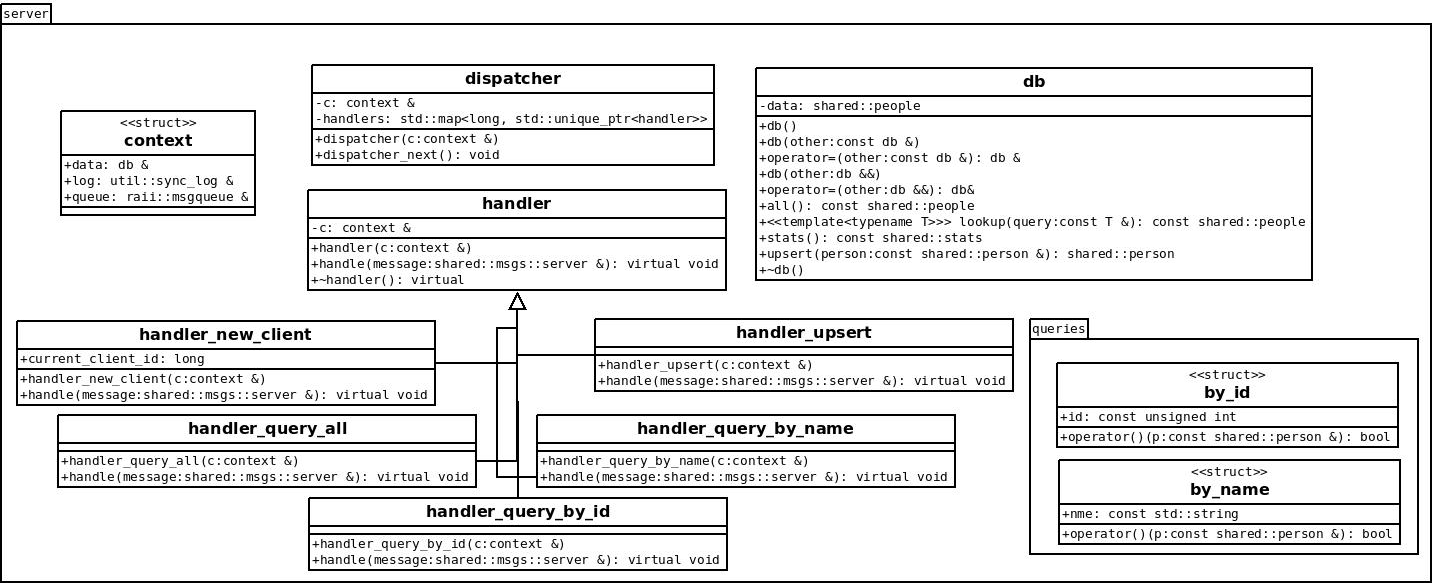
\includegraphics[scale=0.8,angle=90]{server.png}
    \end{center}
\end{figure}

	\clearpage
    
    \subsection{Client}
	\begin{center}
        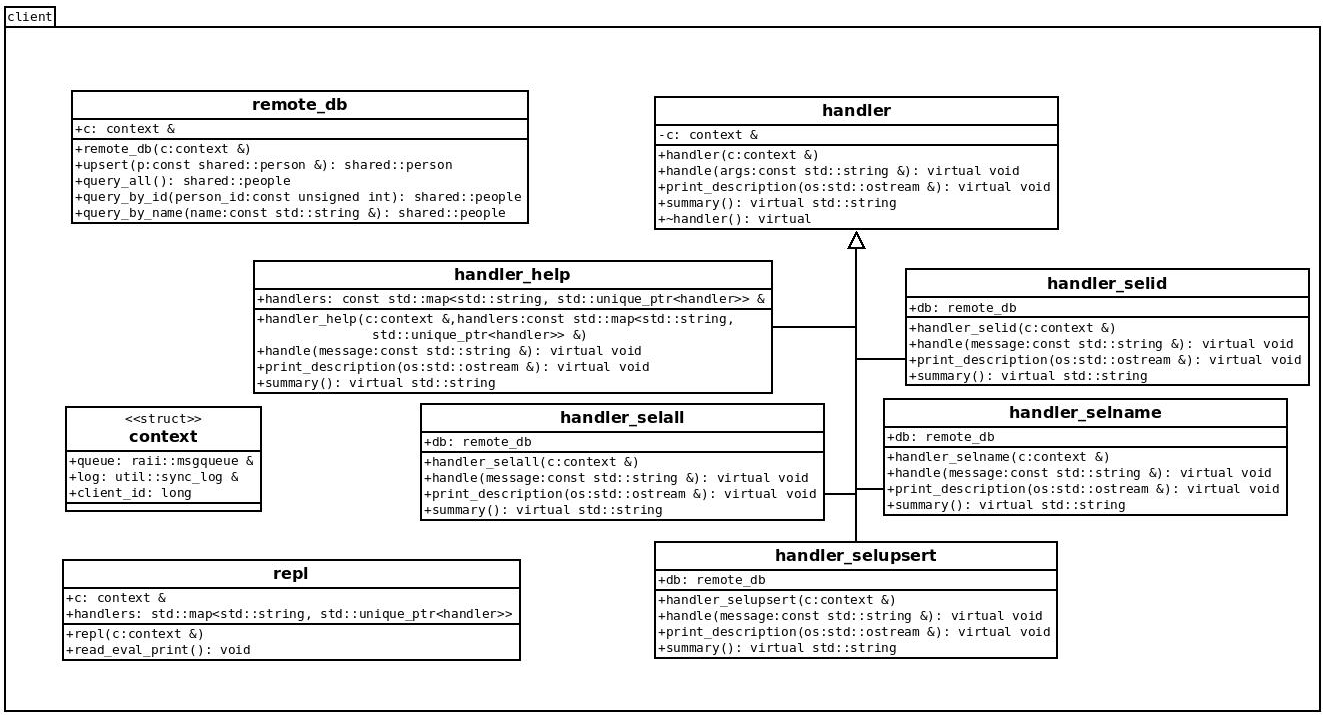
\includegraphics[scale=0.8,angle=90]{client.png}
    \end{center}
    
    \clearpage

    \subsection{Shared}
	\begin{center}
        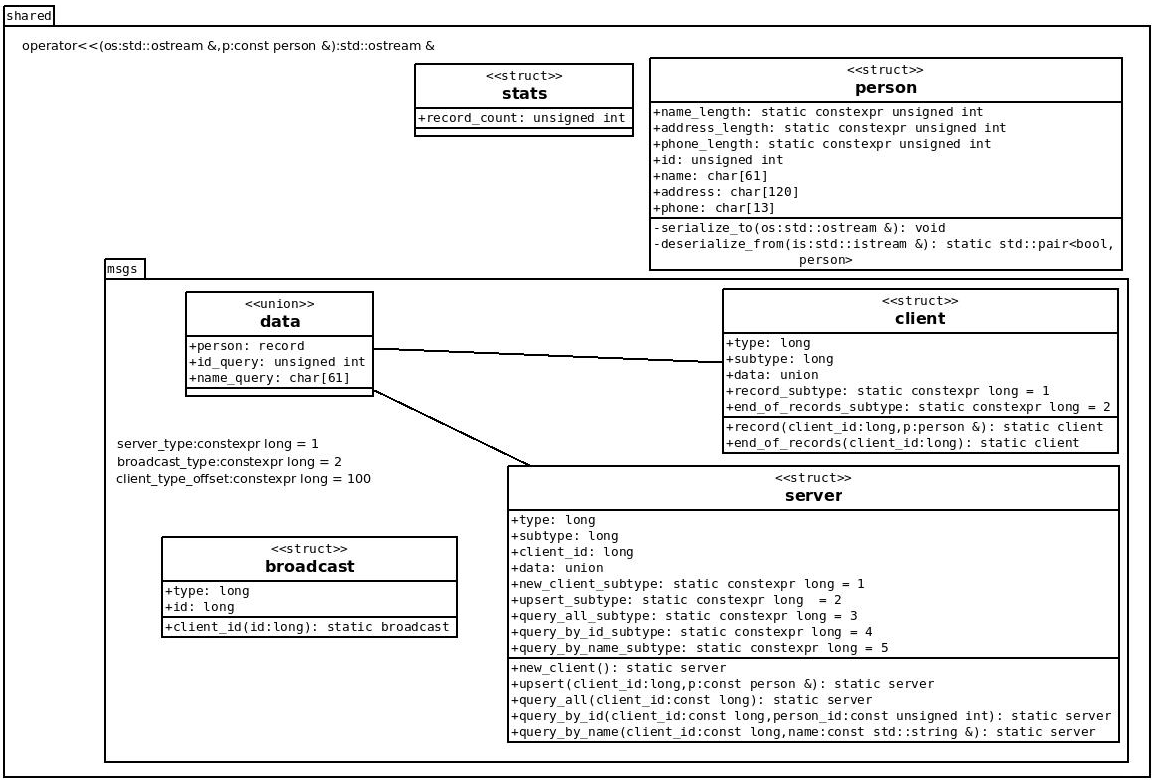
\includegraphics[scale=0.8]{shared.png}
    \end{center}
    
    \subsection{Raii}
	\begin{center}
        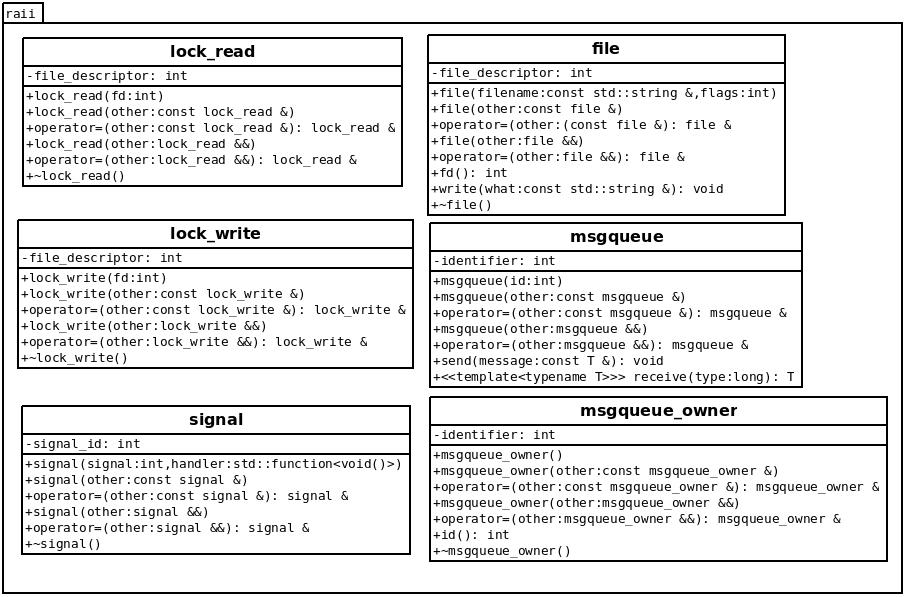
\includegraphics[scale=0.8]{raii.png}
    \end{center}
    
    \subsection{Syscalls}
	\begin{center}
        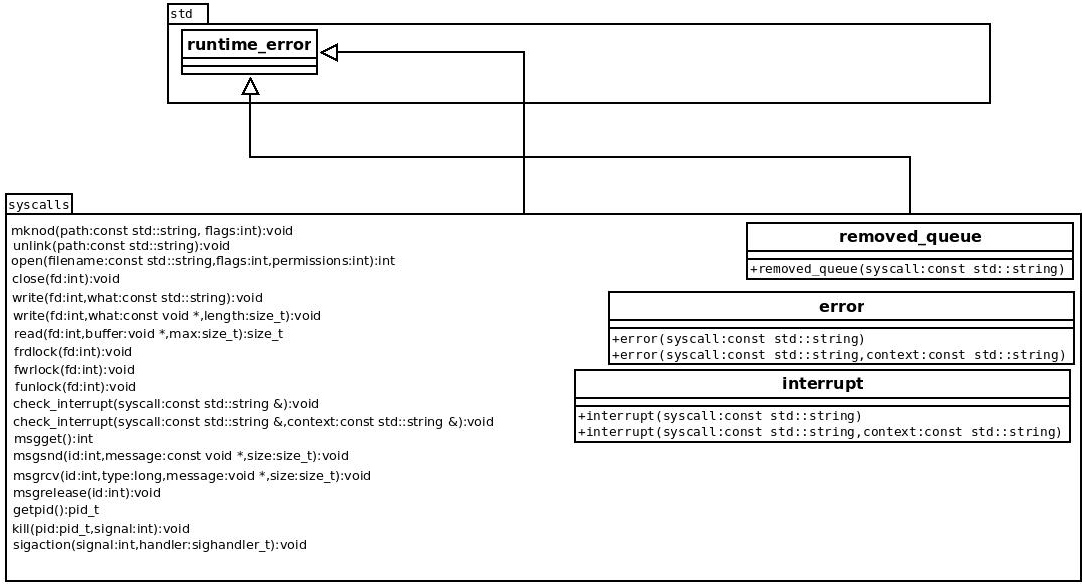
\includegraphics[scale=0.8]{syscalls.png}
    \end{center}

    \subsection{Util}
	\begin{center}
    	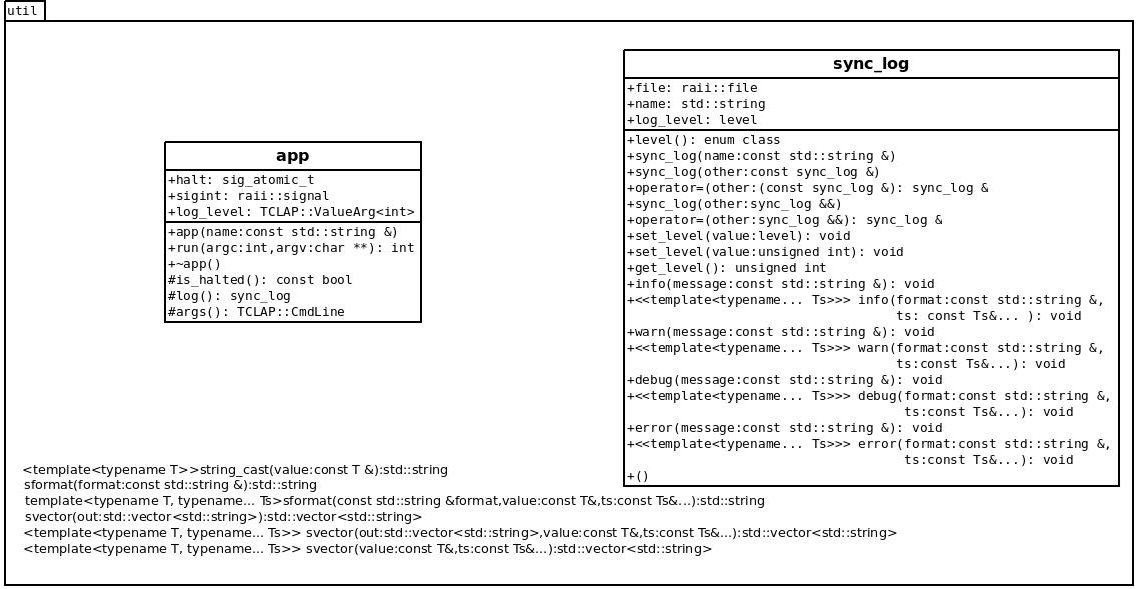
\includegraphics[scale=0.8]{util.png}
    \end{center}
    
\clearpage
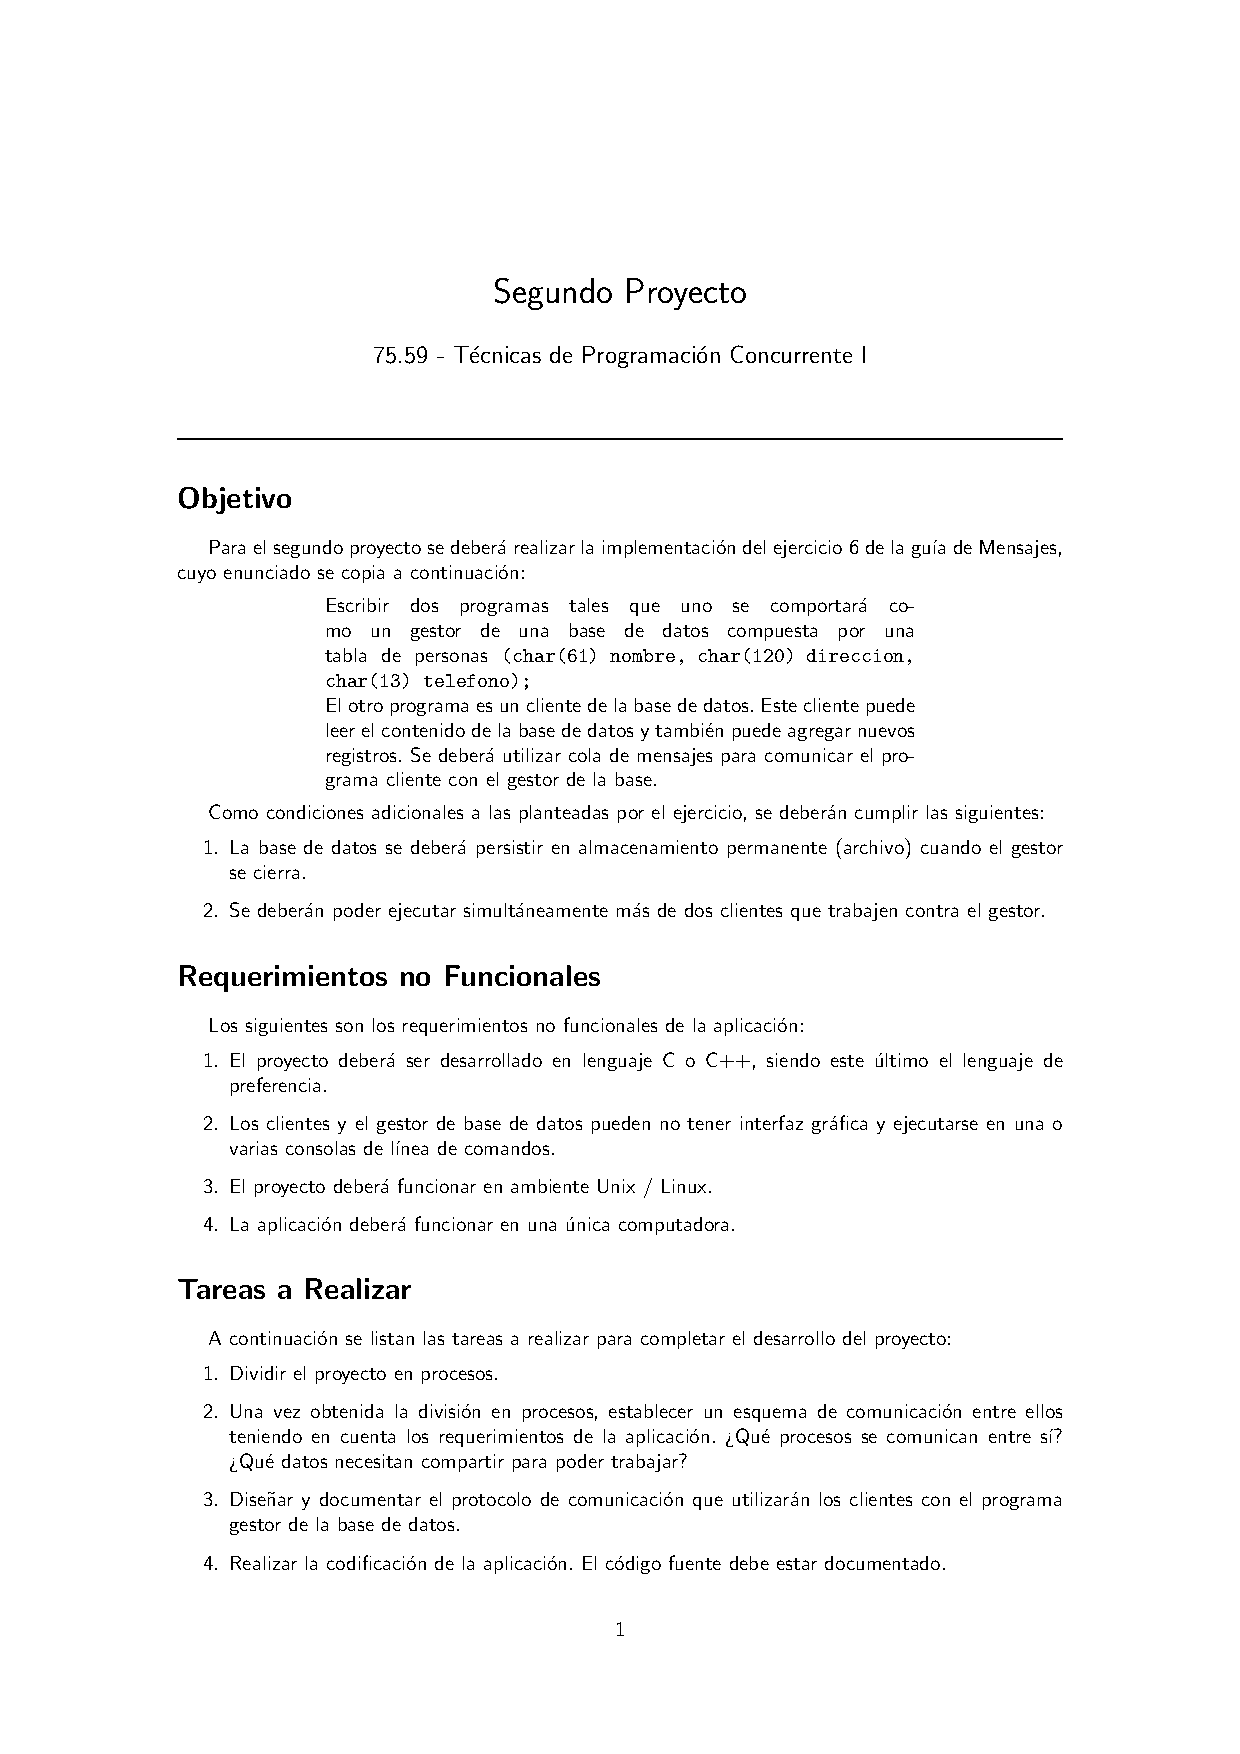
\includepdf[pages={-}]{enunciado.pdf}

\end{document}